\chapter{Modello a Rete}

\begin{center}
	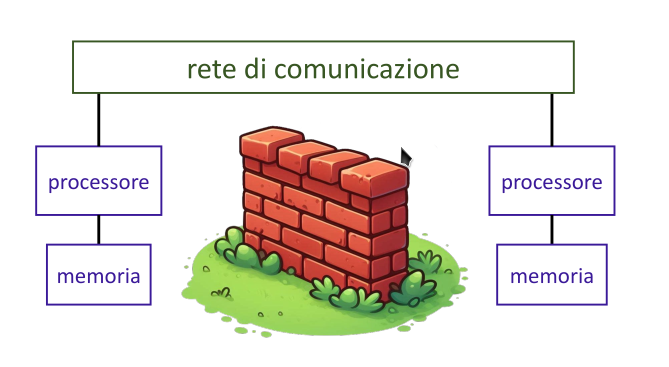
\includegraphics[scale=0.6]{05-Rete/vm.png}
\end{center}
\section{Introduzione}

\paragraph{Aspetti caratterizzanti del modello a rete:}

\begin{itemize}
	\item Ogni processo può accedere esclusivamente alle risorse allocate nella propria \fancyglitter{memoria locale} (eventualmente virtuale), non esiste \fancyglitter{memoria condivisa}.
	\item La comunicazione avviene solo per \fancyglitter{scambio di messaggi}.
	\item Rimane il concetto di \fancyglitter{interleaving}.
\end{itemize}

\subsection{Sistemi Fortemente e Debolmente Connessi}

\dfn{Sistema Fortemente Connesso}{
	Un sistema è fortemente connesso (tightly coupled) se ogni
	componente necessita della completa conoscenza delle
	caratteristiche degli altri componenti del sistema.
}

\cor{RC 4000}{
	RC 4000 era un sistema operativo monoprocessore multiprogrammato progettato alla fine degli anni '60. La memoria non occupata dal nucleo del OS era suddivisa tra i processi attivi.
}

\paragraph{Il kernel associa a ogni processo una coda di messaggi, un pool di buffer per la comunicazione, e 4 primitive di kernel:}

\begin{itemize}
	\item send message(receiver, message, buffer): copia il messaggio in un buffer libero e lo manda al receiver (senza bloccare il mittente).
	\item wait message(sender, message, buffer): attende l’arrivo di un messaggio nella coda del processo.
	\item send answer(result, answer, buffer): copia la risposta nel buffer del mittente e glielo rimanda. Il processo rispondente (sender) non attende la consegna.
	\item wait answer(result, answer, buffer): attende la risposta dal processo che ha ricevuto il messaggio inviato con send message. L’argomento result è un codice di successo/fallimento. Ritorna il buffer usato nel pool dei buffer liberi.
\end{itemize}

\begin{center}
	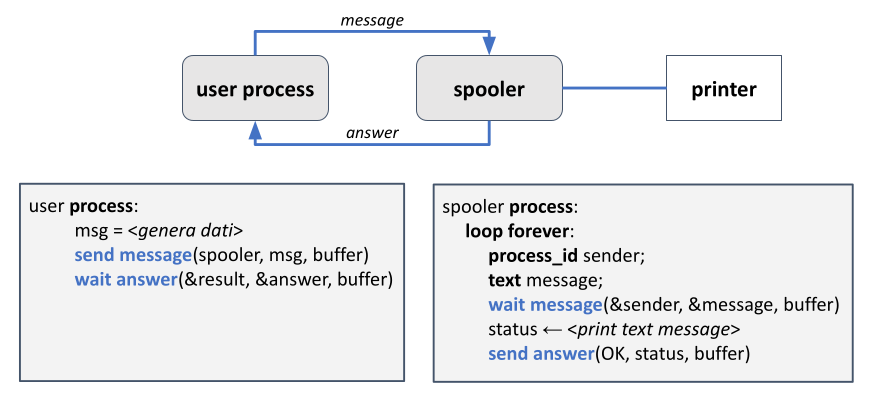
\includegraphics[scale=0.5]{05-Rete/RC4000.png}
\end{center}



\dfn{Sistema Debolmente Connesso}{
	Un sistema è debolmente connesso (loosely coupled) se
	ogni componente necessita di poche o nessuna conoscenza
	delle caratteristiche degli altri componenti del sistema.
}

\subsection{Canali di Comunicazione}

\dfn{Canale}{
	Un canale è un collegamento logico mediante il quale due processi comunicano.
}

\nt{È solitamente compito del nucleo dell'OS fornire l'\fancyglitter{astrazione di canale} come meccanismo primitivo per lo scambio di informazioni.}

\paragraph{Parametri caratterizzanti il canale:}

\begin{itemize}
	\item Il tipo di \fancyglitter{sincronizzazione} tra i processi comunicanti.
	\item La designazione del canale e dei processi \fancyglitter{sorgente} e \fancyglitter{destinatario} di ogni comunicazione (indirizzamento).
	\item La tipologia del canale intesa come \fancyglitter{direzione del flusso di dati} che un canale può trasferire (il canale è unidirezionale).
\end{itemize}

\paragraph{Tipologie di sincronizzazione:}

\begin{itemize}
	\item \fancyglitter{Comunicazione asincrona:}
	      \begin{itemize}
		      \item Il processo sender deposita il messaggio e prosegue.
		      \item Il processo receiver si blocca se non ci sono messaggi nel canale.
		      \item Non c'è sincronizzazione tra processi.
		      \item Necessità di un buffer di messaggi.
	      \end{itemize}
	\item \fancyglitter{Comunicazione sincrona:}
	      \begin{itemize}
		      \item Il processo Receiver si blocca se non ci sono messaggi nel canale.
		      \item Il processo Receiver si blocca se il Sender non è pronto a consegnare il messaggio.
		      \item Lo scambio di messaggi è un mezzo di sincronizzazione tra i processi.
		      \item Non c’è necessità di un buffer di messaggi.
	      \end{itemize}
	\item \fancyglitter{Comunicazione con sincronizzazione estesa (Rendez-vous):}
	      \begin{itemize}
		      \item Il processo Sender aspetta il Receiver, consegna il messaggio e aspetta la risposta.
		      \item Il processo Receiver aspetta il Sender, legge il messaggio e gli consegna la risposta.
		      \item I due processi rimangono sincronizzati fino a che messaggio e risposta non sono consegnati.
	      \end{itemize}
\end{itemize}

\paragraph{Tipi di canale:}

\begin{itemize}
	\item Da uno a uno (link): produttore/consumatore, pipe UNIX, transputer.
	\item Da molti a uno (port): client/server.
	\item Da molti a molti (mailbox).
\end{itemize}

\nt{Inoltre i canali possono essere \fancyglitter{unidirezionali} o \fancyglitter{bidirezionali}.}

\subsection{Dichiarazione di Canali}

\paragraph{port $<$tipo$>$ $<$identificatore$>$:}

\begin{itemize}
	\item Canale da molti a uno.
	\item È tipato ed è denotato da un identificatore.
	\item Ci si accede mediante dot notation.
\end{itemize}

\paragraph{Primitive:}

\begin{itemize}
	\item Invio (send($<$value$>$) to $<$port$>$):
	      \begin{itemize}
		      \item $<$port$>$ identifica  in modo univoco il canale a cui inviare il messaggio.
		      \item $<$value$>$ è il contenuto del messaggio (dello stesso tipo di $<$port$>$).
	      \end{itemize}
	\item Ricezione ($<$proc$>$ = receive($var$) from $<$port$>$):
	      \begin{itemize}
		      \item $<$port$>$ identifica  in modo univoco il canale a cui inviare il messaggio.
		      \item $<$var$>$ è una variabile a cui assegnare il valore del messaggio ricevuto  (dello stesso tipo di $<$port$>$).
		      \item $<$proc$>$ è l'identificatore di una variabile processo a cui viene assegnato l'identificatore del processo mittente.
	      \end{itemize}
\end{itemize}

\nt{
	Queste primitive non permettono di stabilire se la comunicazione è asincrona o sincrona;
	la scelta della realizzazione sincrona o asincrona dipende dal linguaggio di programmazione
	e l’utilizzatore deve esserne a conoscenza.
}


\subsection{Guardie}

\dfn{Guardia}{
	La $<$guardia$>$ è costituita da una coppia ($<$espressione booleana$>$; $<$primitiva receive$>$).
}

\paragraph{La guardia viene valutata e ha tre possibili esiti:}

\begin{itemize}
	\item \fancyglitter{Fallita:} se l'espressione booleana è false.
	\item \fancyglitter{Ritardata:} se l'espressione booleana è true ma la receive è bloccata poiché sul canale su cui viene eseguita non ci sono messaggi pronti.
	\item \fancyglitter{Valida:} se l'espressione booleana è true e la receive può essere eseguita senza ritardi.
\end{itemize}

\paragraph{Comandi con guardie multiple:}

\begin{itemize}
	\item Vengono valutate le guardie di tutti i rami.
	\item Se una o più guardie sono valide viene scelto, in maniera non deterministica,
	      uno dei rami con guardia valida e viene eseguita la receive contenuta nella
	      guardia scelta; viene quindi eseguita l’istruzione relativa al ramo scelto.
	      Successivamente, l’esecuzione dell’intero comando viene ripetuta.
	\item Se tutte le guardie non valide sono ritardate, il processo in esecuzione si
	      sospende in attesa che arrivi un messaggio che abilita la transizione di una
	      guardia da ritardata a valida.
	      A quel punto procede come nel caso precedente.
	\item Se tutte le guardie sono fallite l’esecuzione del blocco do..od (guardie multiple) termina.
\end{itemize}

\section{Comunicazione Sincrona}

\subsection{Transputer}

\cor{Transputer}{
	Il termine Transputer identifica una famiglia di micro-computer costituiti da un unico chip contenente: \begin{itemize}
		\item Un processore con memoria propria.
		\item Quattro canali unidirezionali.
	\end{itemize}
}

\begin{center}
	\begin{minipage}{0.45\textwidth}
		\centering
		
\includegraphics[scale=0.25]{05-Rete/tboy.png}
	\end{minipage}%
	\hfill
	\begin{minipage}{0.45\textwidth}
		\centering
		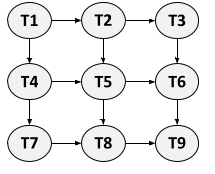
\includegraphics[scale=0.7]{05-Rete/transputer.png}
	\end{minipage}
\end{center}

\clm{}{}{
	\begin{itemize}
		\item La comunicazione è \fancyglitter{sincrona}, mediante istruzioni in linguaggio macchina.
		\item I quattro canali unidirezionali permettono l'interconnessione con altri transputer (link).
		\item Processi statici.
	\end{itemize}
}

\paragraph{Moltiplicazione parallela di matrici:}

\begin{itemize}
	\item Passare un elemento $x$ da NORD.
	\item Passare $x$ a SUD immodificato.
	\item Moltiplicare $x$ per $val$.
	\item Prendere il valore somma parziale $p$ da EST.
	\item Sommare $p$ a $x*val$.
	\item Mandare il risultato a OVEST.
\end{itemize}

\begin{center}
	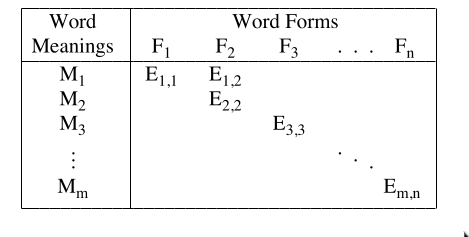
\includegraphics[scale=0.36]{05-Rete/matrix.png}
\end{center}

\nt{Nei linguaggi dedicati ai transputer (CSP, OCCAM,\dots) erano stati introdotti comandi selettivi.}

\begin{center}
	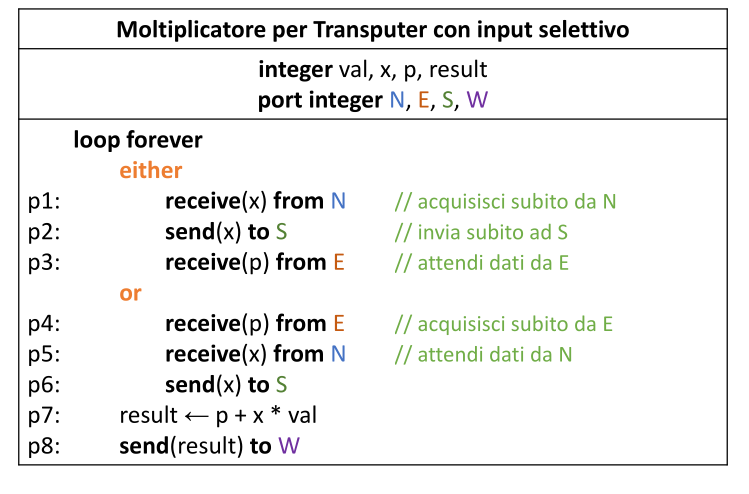
\includegraphics[scale=0.36]{05-Rete/matrix2.png}
\end{center}

\subsection{Canali Sincroni - Pipe}

\dfn{Problema di Conway}{
	Nei sistemi operativi i canali sono chiamati pipe e sono usati per collegare insiemi di
	programmi esistenti. Come esempio di una computazione concorrente con pipe
	consideriamo una variante del problema di Conway (run-length compression):
	\begin{itemize}
		\item L’input è una sequenza di caratteri inviati da un ambiente esterno a un canale di
		      input inC.
		\item L’output è la stessa sequenza mandata ad un ambiente esterno tramite un canale
		      outC dopo aver eseguito due trasformazioni:
		      \begin{itemize}
			      \item Le $n (2 \leq n \leq 9)$ occorrenze consecutive di un carattere char sono sostituite dalla coppia $<n$, char$>$.
			      \item Nella sequenza di output viene inserita un ritorno\_a\_capo dopo K caratteri
		      \end{itemize}
	\end{itemize}
}

\begin{center}
	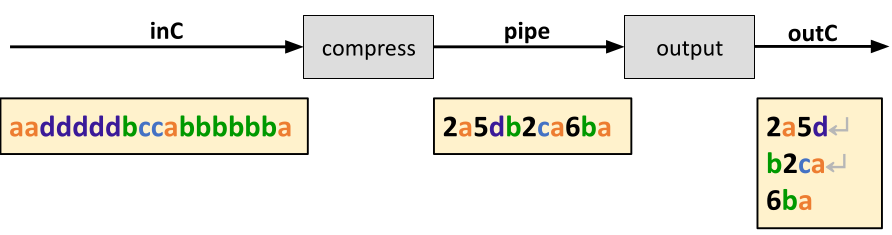
\includegraphics[scale=0.46]{05-Rete/conway.png}
\end{center}

\begin{center}
	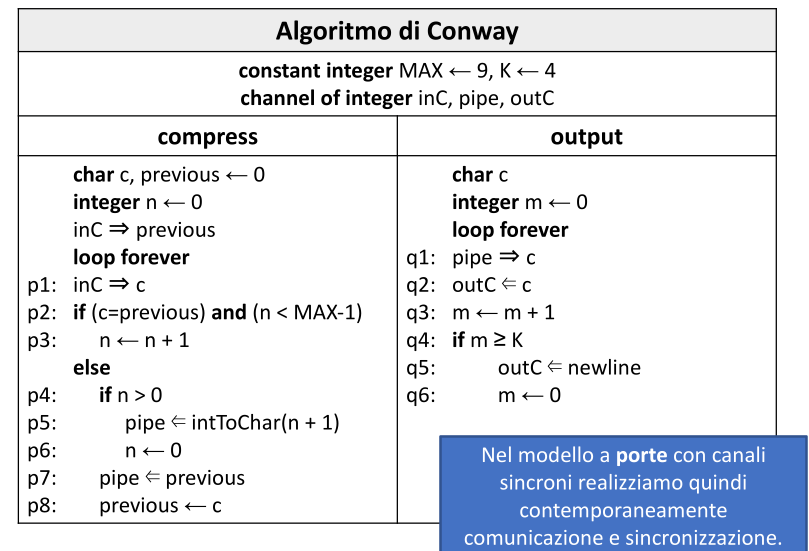
\includegraphics[scale=0.4]{05-Rete/calg.png}
\end{center}

\section{Rendez-vous e RPC}

\subsection{Rendez-vous}

\dfn{Rendez-vous}{
	l processo server specifica le operazioni che offre un servizio come una
	sequenza di istruzioni che può comparire in un punto qualunque del suo
	codice. Utilizza un’istruzione di input (accept) che lo sospende in attesa di
	una richiesta dell’operazione da parte dei client. All’arrivo della richiesta il
	processo server esegue il relativo insieme di istruzioni e invia al client
	chiamante i risultati.
}

\clm{}{}{
	\begin{itemize}
		\item Meccanismo di comunicazione e sincronizzazione tra processi in cui un
		      processo che richiede un servizio a un altro processo rimane sospeso
		      fino al completamento del servizio richiesto (meccanismo sincrono).
		\item I processi rimangono sincronizzati durante l’esecuzione del servizio da
		      parte del ricevente (\fancyglitter{processo accettante}) e fino alla ricezione dei
		      risultati da parte del mittente (\fancyglitter{processo chiamante}).
		\item Il processo accettante non deve conoscere l’identità del processo
		      chiamante, così il rendezvous è particolarmente utile per gestire i
		      rapporti client/server (meccanismo asimmetrico)
		\item Analogia semantica con una normale chiamata di funzione. Il
		      programma chiamante prosegue solo dopo che l’esecuzione della
		      funzione è terminata. La differenza sostanziale sta nel fatto che la funzione (servizio) viene
		      eseguita remotamente da un processo diverso dal chiamante.
	\end{itemize}
}

\paragraph{Sintassi:}

\begin{itemize}
	\item entry $<$servizio$>$ (in $<$par-ingresso$>$, out $<$par-uscita$>$): processo che offre un servizio.
	\item accept $<$servizio$>$ (in $<$par-ingresso$>$, out $<$par-uscita$>$) \{$<$codice del servizio $>$\} $\rightarrow$ $<$codice post sincronizzazione $>$: accettazione di nuove richieste:
	      \begin{itemize}
		      \item \fancyglitter{Servizio:} il client è in attesa della risposta.
		      \item \fancyglitter{Post sincronizzazione:} la sincronizzazione con il client è terminata ma il server può ancora fare delle operazioni.
		      \item Si possono usare le guardie per selezionare le richieste da servire.
	      \end{itemize}

\end{itemize}

\cor{ADA}{
	Il linguaggio ADA, sviluppato per conto del Department of Defense (DOD) degli USA, adotta come metodo di interazione tra i processi il rendezvous.
}

\paragraph{Rendez-vous in ADA:}

\begin{itemize}
	\item Una entry definita in un task P può essere chiamata da un altro task Q.
	\item Lo schema base di un task contiene una parte di specifica
	      che definisce le operazioni entry e una parte body che
	      consente la realizzazione di tali operazioni.
	\item Possono essere utilizzati per implementare semafori.
\end{itemize}

\subsection{RPC}

\dfn{Remote Procedure Call (RPC)}{
	Per ogni operazione che un processo client può richiedere, viene dichiarata,
	lato server, una procedura. In esecuzione, per ogni nuova richiesta di
	operazione, viene avviato un nuovo processo (thread) servitore con il
	compito di eseguire la procedura corrispondente.
}

\nt{
	RPC rappresenta esclusivamente un meccanismo di
	comunicazione tra processi; la possibilità che più
	operazioni siano eseguite concorrentemente da thread
	diversi comporta che si debba provvedere separatamente
	a una sincronizzazione tra processi servitori.
}


\begin{center}
	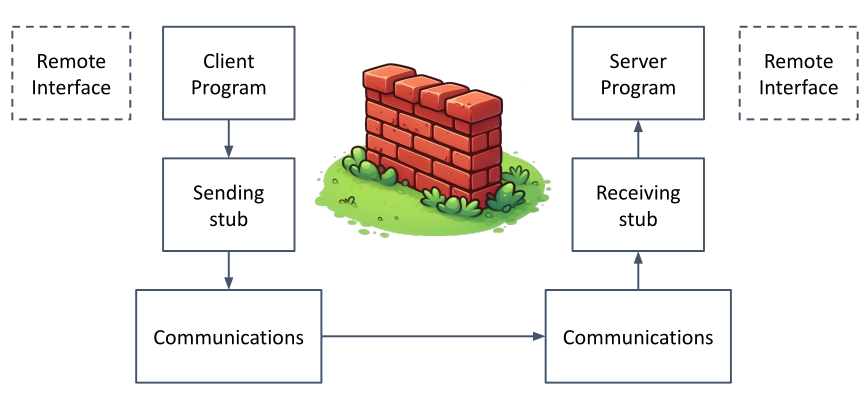
\includegraphics[scale=0.4]{05-Rete/rpc.png}
\end{center}

\clm{}{}{
	\begin{itemize}
		\item L'insieme delle procedure remote è definito all'interno di un componente sw (modulo), che
		      contiene anche le variabili locali al server ed eventuali procedure e processi locali.
		\item I singoli moduli operano in spazi di \fancyglitter{indirizzamento diversi} e possono quindi essere
		      allocati su nodi distinti di una rete.
		\item Il server crea un thread che esegue l'operazione richiesta.
		\item In ogni stato è possibile che più thread concorrenti
		      all'interno del modulo accedano a variabili interne.
		\item Necessità di sincronizzazione mediante semafori, monitor, \dots
	\end{itemize}
}


